\section{Experimental Setup}
    \subsection{Environment}
        We use the Farama Gymnasium's Ant-v4 environment \cite{Gymnasium2023} to evolve generalist MC-pairs. This environment consists of a flat plane for the ant to walk on, with the objective of traversing a long distance. The ant's morphology comprises of four legs, each composed of an upper and a lower leg, with the upper leg attached to the torso. Figure~\ref{fig:ant_env} shows the appearance of the ant. 
        \begin{figure}[ht]
            \centering
            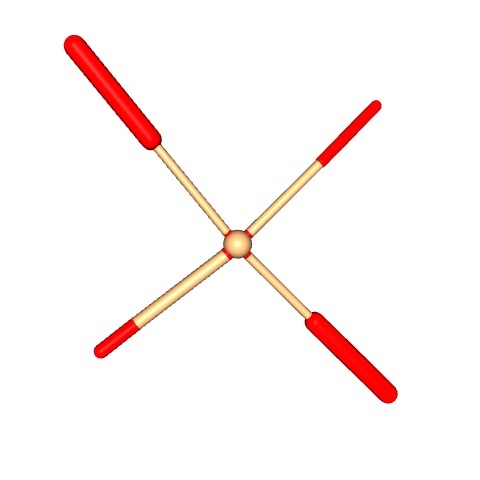
\includegraphics[width=0.9\linewidth]{./resources/ant_307.png}
            \caption{Example of an ant in the environment. The red legs depict the lower leg part, and the light beige represents the upper leg part.}
            \label{fig:ant_env}
        \end{figure}
        To evolve a generalist MC-pair, we have to enable the ant to modify its morphology. Each leg part is parameterized by two attributes: length and width, resulting in a total of 16 distinct morphological parameters. The leg lengths are constrained between 0.1 and 1.5, while the widths are limited from 0.08 to 0.2. 
        
        To ensure a fast and successfull experiment, additional modifications to the ant's environment were necessary. Normally, the simulation would terminate the when the ant's torso ascends or descends to a specific height. This range has been increased to allow the ant to grow longer legs. Furthermore, additional settings were introduced to terminate the run whenever no significant forward movement was detected, suggesting that the ant had frozen in place. Another custom rule was implemented to detect if the ant flipped upside down by monitoring the z-vector of the torso. These additions significantly reduced evaluation times, especially at the start of the evolutionary process.

    \subsection{Experimental parameters}
        For the controller, a fully connected feedforward ANN is evolved, based on the topology used by Triebold et al. \cite{Corinna_Triebold}. This topology consists of a single hidden layer with 20 neurons. The input layer corresponds to the ant's continuous observation space, which includes 27 observations, such as the angles between the torso and leg connections or velocity values, resulting in 27 input nodes. The output layer corresponds to the ant's action space, where actions are values ranging from [-1, 1], representing the torque applied to the rotors. This results in a total of 8 actions and thus 8 output nodes. Each layer also includes a bias node.
        
        For the parameters used in the XNES algorithm, we used the default settings provided by the algorithm. The initial standard deviation of the search was set to 0.01, and the initial parameter ranges for the controller and encoded morphology parameters were [-0.1, 0.1]. To decode the morphology parameters, a linear transformation is used where the lower bound morphology constraint maps to -0.1 and the upper bound morphology constraint maps to 0.1. The lower and upper bound constraints used for the length and width of the legs are [0.1, 1.5] [0.05, 0.2] respectively. \textbf{Should I also insert these linear transformation formula's that I used specifically?}
        
        The parameters used for the penalty function were decided based on initial experimental analysis. For the growth rate $r^i$, we settled on 1.03 in conjunction with two scale factors for $\alpha$. This means we are using two different penalty functions. The reason for this is that when the morphological parameters are decoded into negative values, the environment will crash because it cannot accommodate negative values for morphology. In these cases, $\alpha$ is set to 1000; otherwise, it is set to 100.
        
        For the evolutionary process, we decided to evaluate the generalist scores after 2500 generations, instead of at every generation from the start. The reason for this is to decrease computational cost, but primarly because at the start of the evolutionary process, it is difficult to achieve high fitness scores due to the search for an effective morphology to exploit. After 2500 generations, a generalist score will be computed from the fittest individual in each generation. If there is no improvement found after 500 generations, the process is either terminated or a partition will occur.

        Additionaly, we conducted an alternative evolutionary run in which partitioning was disabled, allowing the run to extend to 5000 generations. The reason for this is because the of the unpredictability of discovering a generalist MC-pair, due to it not being the objective function, but a secondary outcome of the method used. The exclusion of paritioning in this scenario will provide a valuable basis for comparison with the partitioned approach.
    \subsection{Training, evaluation and testing}
        The MC-pair's training consists of different simulated environments, where the terrain is algorithmically generated based on the inputs. In this experiment, we consider three different environments. The first environment, referred to as the default environment, is a single static environment with a flat surface. The two remaining environments are dynamically generated, named the rough terrain environment and the hill terrain environment (see Figure~\ref{fig:rough_terrain} and Figure~\ref{fig:hills_terrain}, respectively). The rough terrain environment is generated based on the block size and floor height. The block size determines the size of a block that can be elevated, and the floor height determines the range at which this block can be elevated. For the hill terrain environment, we utilize a Perlin noise map to determine the elevations of the terrain. The scale parameter determines the smoothness of the terrain, meaning that the terrain heights have smaller and subtler changes in height, leading to a more hilly terrain, with the floor height serving as the range at which these heights can be set. 
        \begin{figure}[ht]
            \centering
            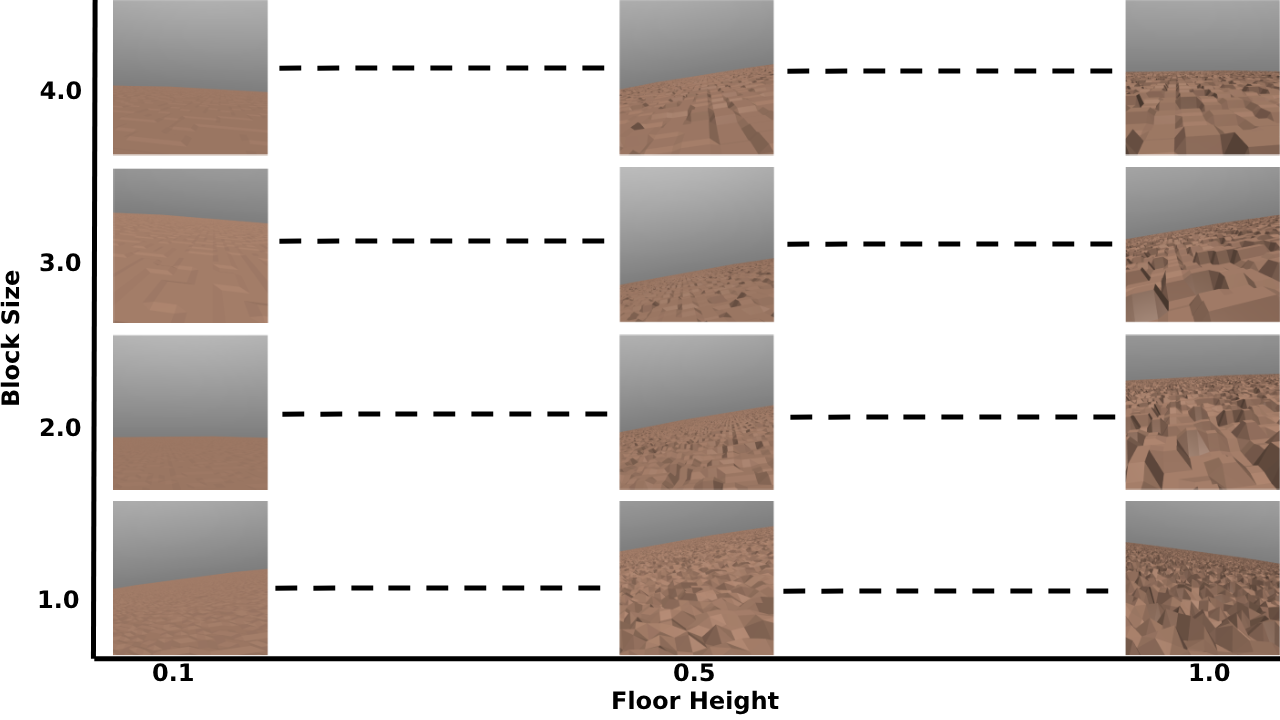
\includegraphics[width=\linewidth]{./resources/rough_terrain.png}
            \caption{Rough terrain environment generation, based on the block size and floor height.}
            \label{fig:rough_terrain}
        \end{figure}
        \begin{figure}[ht]
            \centering
            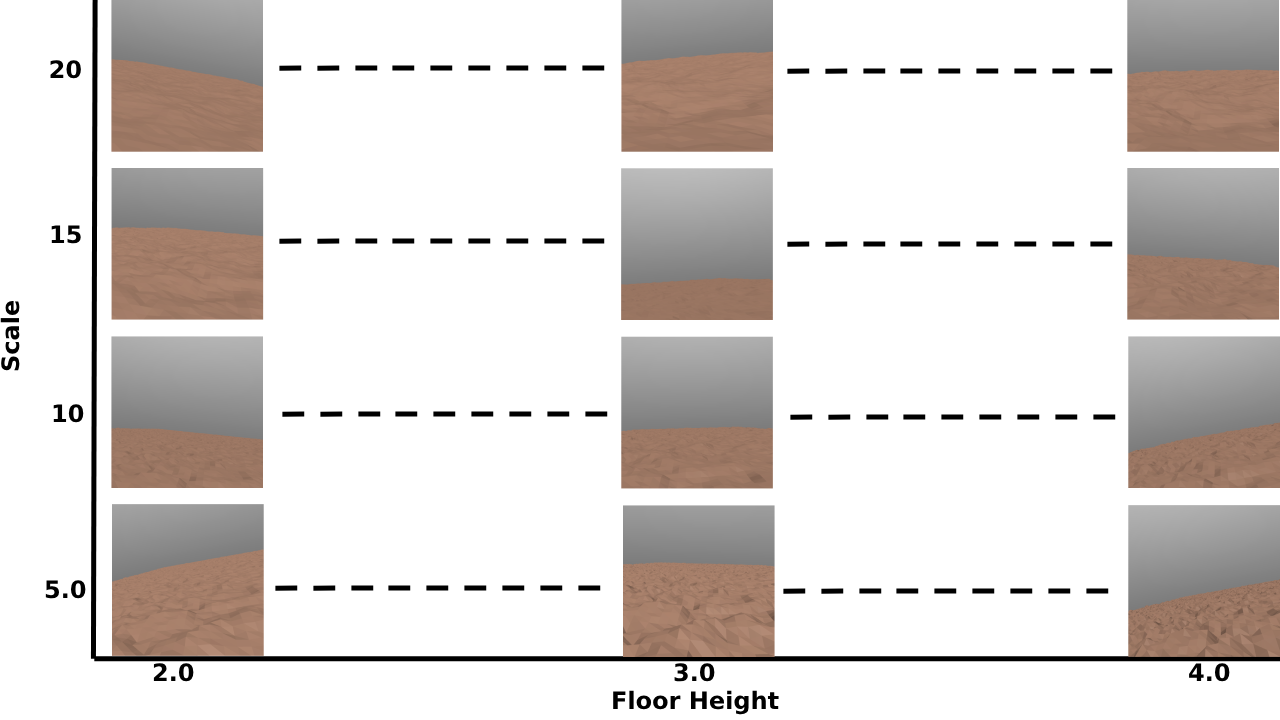
\includegraphics[width=\linewidth]{./resources/hills_terrain.png}
            \caption{Hills terrain environment generation, based on the scale of the Perlin noise and floor height.}
            \label{fig:hills_terrain}
        \end{figure}

        In total, we have 40 variations of the rough terrain environment, 44 variations of the hill terrain environment, and the default environment, totaling up to a set of 85 different environments. We will split this set into training, validation, and testing sets. In our case, for the validation set, we will use the same set as for the training set. The training set contains the default environment, 24 hill environments, and 24 rough terrain environments, totaling to 49 environments. The testing set contains 20 hill environments and 16 rough terrain environments, totaling to 36 environments. The exact splits are shown in Table~\ref{tab:split_table}.

        To test the generalizability of the MC-pair, we run two separate tests. The first test is to evaluate the performance on environments similar to those of training, with both the testing and training environment parameters drawn from the same distribution, which we call interpolation. The second test is to evaluate the performance on environments different from those of training, with the testing and training environment parameters drawn from separate distributions, which we call extrapolation. In summary, to test interpolation, we will utilize the training set, and to test extrapolation, we will use the testing set described in Table~\ref{tab:split_table}.

        \begin{table*}[ht]
            \centering
            \caption{This table shows the environment set splits and used ranges for the hill and rough environments.}
            \begin{tabular}{|c|c|c|c|c|}
            \hline
            \textbf{Environment} & \textbf{Parameters} & \textbf{Training Set} & \textbf{Testing Set} & \textbf{Step} \\ \hline
                Rough terrain & 
                \makecell{Block size \\ Floor height} & 
                \makecell{$[1, 4]$ \\ $[0.2, 0.4] \cup [0.7, 0.9]$} & 
                \makecell{$[1, 4]$ \\ $[0.1] \cup [0.5, 0.6] \cup [1.0]$} & 
                \makecell{1 \\ 0.1}
            \\ \hline
                Hills terrain &
                \makecell{Scale \\ Floor height} & 
                \makecell{$[5, 20]$ \\ $[2.2, 2.6] \cup [3.4, 3.8]$} & 
                \makecell{$[5, 20]$ \\ $[2.0] \cup [2.8, 3.2] \cup [4.0]$} & 
                \makecell{5 \\ 0.2}
            \\ \hline
        \end{tabular}
        \label{tab:split_table}
        \end{table*}